% Author: Alfredo Sánchez Alberca (asalber@ceu.es)
\chapter{Introducción a Derive}

\section{Introducción}
La gran potencia de cálculo alcanzada por los ordenadores en las
últimas décadas, ha convertido a los mismos en poderosas
herramientas al servicio de todas aquellas disciplinas que, como las
matemáticas, requieren cálculos largos y complejos.

Derive$^{\textsf{\textregistered}}$
\renewcommand{\thefootnote}{\fnsymbol{footnote}}\footnote{Esta
practica está basada en la versión 6.1 de
Derive$^{\textregistered}$ para Windows en castellano.} es uno de
los programas de cálculo numérico y simbólico más utilizados.
Aparte de sus capacidades el cálculo numérico, vectorial y
matricial, también permite realizar representaciones gráficas, lo
cual permite resolver multitud de problemas de álgebra, análisis,
cálculo, geometría e incluso estadística. La ventaja de Derive
frente a otros programas habituales de cálculo como Mathematica,
Mapple o MATLAB, radica en su sencillez y simplicidad de uso, lo
cual lo hace idóneo para la enseñanza de las matemáticas.

\begin{center}
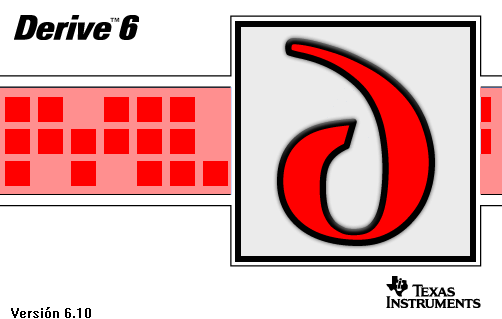
\includegraphics[scale=0.6]{img/introduccion_derive/introduccion}
\end{center}


El objetivo de esta práctica es introducir al alumno en la
utilización de este programa, enseñándole a realizar las operaciones
básicas más habituales.


\section{Funciones básicas}
\subsection*{Arranque}
Como cualquier otra aplicación de Windows, para arrancar el programa
hay que pulsar sobre la opción correspondiente del menú
\menu{Inicio>Programas}, o bien sobre el icono de escritorio


\begin{center}

\includegraphics[scale=0.4]{img/introduccion_derive/icono}
\end{center}

Cuando el programa arranca, en la pantalla aparece la ventana
principal del programa que se conoce como \emph{ventana de Álgebra}
(figura \ref{g:principal}).

\begin{figure}[h!]
\begin{center}
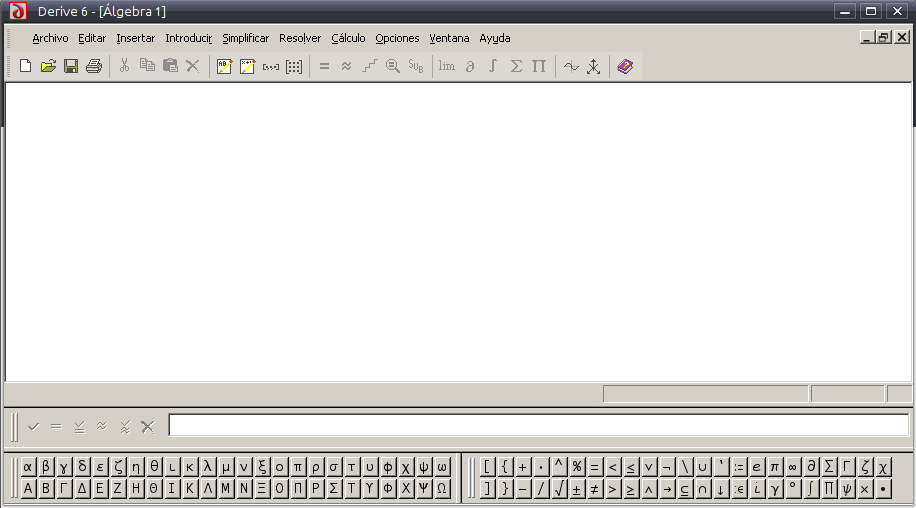
\includegraphics[scale=0.6]{img/introduccion_derive/principal}
\caption{Ventana principal de Derive.} \label{g:principal} 
\end{center}
\end{figure}


Como cualquier otra ventana de aplicación de Windows, la ventana
principal tiene una barra de título, una barra de menús con las
distintas funciones que puede hacer Derive (cálculo de límites,
derivadas, integrales, representaciones gráficas, etc.), una barra
de botones que son atajos a las opciones más habituales de los
menús, y una barra de estado en la parte inferior que nos indica lo
que hace el programa en cada instante. Además, por defecto, en la
parte inferior de la ventana aparece el editor de expresiones, que
pasamos a describir a continuación.

\subsection*{Edición de expresiones}
Antes de realizar cualquier cálculo sobre una expresión matemática,
lo primero es escribir dicha expresión y aprender a manipularla.
\subsection*{Introducción de expresiones}
Para introducir una expresión se utiliza el editor de expresiones
(figura~\ref{g:editor}), el cual aparece directamente en la parte
baja de la ventana de Álgebra.
\begin{figure}[h!]
\begin{center}
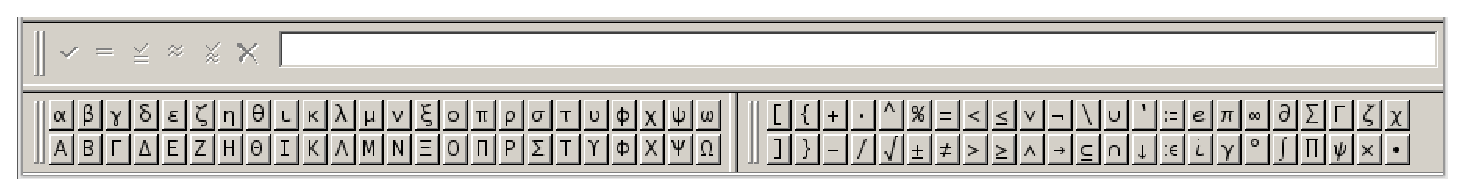
\includegraphics[scale=0.6]{img/introduccion_derive/authorexpression}
\caption{Editor de expresiones.} \label{g:editor} 
\end{center} 
\end{figure}

El editor de expresiones está compuesto por una línea de edición,
que se utiliza para dar forma a las expresiones matemáticas (también
permite introducir comentarios de texto) que vamos a utilizar con el
programa, una barra con las letras del alfabeto griego, a menudo
presentes en las expresiones matemáticas, y una barra de símbolos
matemáticos con los operadores más habituales (suma, resta,
producto, división, paréntesis, raíz cuadrada) y las constantes que
más se utilizan (número $e$, número $\pi$...).

En el editor de expresiones podemos escribir números, letras (que
serán variables), símbolos y operadores aritméticos y relacionales.
Los operadores más habituales en la construcción de expresiones son
los que aparecen en la siguiente tabla:

\begin{center}
\begin{tabular}{|c|c|}
\hline
 Símbolo &   Operador   \\
\hline\hline
    \texttt{+}    &     suma     \\
\hline
    \texttt{-}    &    resta     \\
\hline
    \texttt{*}    &   producto   \\
\hline
    \texttt{/}    &   cociente   \\
\hline
   \texttt{\^{}}    & potenciación \\
\hline
\end{tabular}
\end{center}

A la hora de escribir una expresión hay que tener en cuenta que
Derive tiene establecido un orden de prioridad en la evaluación de
los operadores. En primer lugar evalúa las funciones y constantes
predefinidas, después evalúa las potencias, después productos y
cocientes (ambos con igual prioridad y de izquierda a derecha), y
por último sumas y restas (ambas con igual prioridad y de izquierda
a derecha). Para forzar la evaluación de una subexpresión,
saltándose el orden de evaluación de Derive, se utilizan paréntesis.
Así, como se ve en el siguiente ejemplo, dependiendo de cómo se
introduzca una expresión pueden obtenerse resultados diferentes.

\begin{center}\renewcommand{\arraystretch}{2}
\begin{tabular}{|c|c|}
\hline
  Expresión introducida & Expresión resultante \\
\hline\hline
        \texttt{4x-1/x-5}        & $4x-\dfrac{1}{x}-5$ \\
\hline
       \texttt{(4x-1)/x-5}       & $\dfrac{4x-1}{x}-5$  \\
\hline
       \texttt{4x-1/(x-5)}       & $4x-\dfrac{1}{x-5}$  \\
\hline
      \texttt{(4x-1)/(x-5)}      & $\dfrac{4x-1}{x-5}$  \\
\hline
\end{tabular}
\end{center}

Cada vez que introducimos una expresión, esta aparece en la ventana
de Algebra etiquetada con un número precedido del símbolo de
almoadilla \verb"#", tal y como se muestra en la
figura~\ref{g:expresiones}. Posteriormente, cada vez que queramos
hacer referencia a dicha expresión podremos utilizar su etiqueta en
lugar de volver a escribir la expresión.

Es posible seleccionar cualquier expresión o subexpresión de la
ventana Algebra con el ratón o bien con las teclas del cursor.

La tecla \texttt{F3} permite introducir la expresión que tengamos
seleccionada en el editor de expresiones.

\subsubsection*{Modificación de expresiones}
Una vez introducida una expresión, podemos volver a editarla para
realizar cualquier corrección o cambio mediante el menú
\menu{Editar>Expresión} y aparecerá la ventana del editor de
expresiones con la expresión seleccionada.
\subsubsection*{Eliminación de expresiones}
Para eliminar una expresión de la ventana de Algebra, basta con
seleccionarla y utilizar el menú \menu{Editar>Borrar} y la
expresión seleccionada desaparecerá automáticamente, mientras que el
resto de las expresiones se renumeran automáticamente. También es
posible eliminar bloques completos de expresiones consecutivas
seleccionando previamente el bloque de expresiones a eliminar.

\textbf{¡Importante!}: Si hemos eliminado alguna expresión por
equivocación, es posible recuperarla mediante el menú
\menu{Editar>Recuperar}.

\subsubsection*{Reordenación de expresiones}
Es posible cambiar la posición que ocupa una expresión en la ventana
de Álgebra marcándola y arrastrándola mediante el ratón hasta la
posición que queremos que ocupe. Al cambiar la posición de una
expresión, inmediatamente se renumeran las expresiones de la ventana
de Álgegra.

\subsubsection*{Introducción de comentarios}
Hay dos formas diferentes para introducir un comentario en la
secuencia de expresiones. La primera consiste en utilizar la línea
de edición escribiendo el texto del comentario entre comillas, y,
si procedemos de esta manera, el comentario aparecerá como una
expresión más, con su correspondiente etiqueta de ordenación. La
segunda es mediante el menú \menu{Insertar>Objeto de Texto}, y
de esta forma el comentario aparece sin etiqueta de ordenación ya
que se trata de un objeto más insertado en el archivo, como
también lo sería una gráfica, un dibujo, una fotografía o una hoja
de cálculo...

\subsubsection*{Nombres de variables}
Por defecto Derive utiliza una sola letra para representar una
variable, de manera que la expresión \texttt{xy}, no se interpreta
como una variable de nombre $xy$, sino como el producto de la
variable $x$ por la variable $y$. Además, por defecto, no
distingue entre mayúsculas y minúsculas. Por ejemplo, Derive
interpretará que queremos trabajar con la función coseno tanto si
introducimos en la línea de edición $\cos(x)$ como si introducimos
$\cos(X)$. No obstante, es posible hacer que el programa utilice
variables con más de una letra y distinga entre mayúsculas y
minúsculas mediante el menú \menu{Opciones>Ajustes de
Modo>Introducción}.

\subsubsection*{Definición de constantes y funciones}
Es posible definir constantes y funciones mediante el operador de
definición \texttt{:=}. Para definir una constante basta con
escribir el nombre de la constante seguido de \texttt{:=} y el
valor de dicha constante. Por ejemplo para definir la constante de
la aceleración de la gravedad, escribiríamos \texttt{g:=9.8}. Por
otro lado, para definir una función se escribe el nombre de la
función seguido de la lista de variables de la misma separadas por
comas y entre paréntesis; después se escribe \texttt{:=} y por
último la expresión que define la función. Así, por ejemplo, para
definir la función que calcula el área de un triángulo de base $b$
y altura $h$, escribiríamos \texttt{a(b,h):=(b*h)/2} (ver
figura~\ref{g:expresiones}).

Con respecto a la definición de funciones, o de constantes,
resultan especialmente \textbf{¡Importantes!} dos matizaciones:

\begin{itemize}

\item Si hemos definido una función o una constante, la definición
permanece activa durante toda la sesión de trabajo con el
documento, incluso si borramos la expresión en la que hemos
procedido a la definición (al borrar en la pantalla no borramos la
memoria interna en la que se almacenan las definiciones de las
constantes y funciones). Para cambiar una definición previa no
quedará más remedio que redefinir (g:=9.812 ), o dejar la
asignación en blanco si lo que queremos es borrar la definición
(g:= ).

\item En las definiciones de funciones sí que, por defecto, Derive
distingue entre minúsculas y mayúsculas. De tal forma que, por
ejemplo, distinguirá entre $a(b,h)$ y $A(b,h)$.

\end{itemize}

\subsubsection*{Funciones y constantes predefinidas} Derive tiene ya
implementadas la mayoría de la funciones elementales y constantes
que suelen utilizarse en los cálculos matemáticos. La sintaxis de
algunas de estas funciones y constantes se muestra en la
tabla~\ref{t:funcioneselementales}, aunque, muy a menudo, en lugar
de utilizar dicha sintaxis se utilizan los operadores y constantes
que aparecen en la barra de símbolos. Por ejemplo, se puede
observar cómo cambia el aspecto de la letra \texttt{e} introducida
en la línea de edición como un variable más, o si en su lugar
utilizamos \verb"#"\texttt{e}, o la \emph{e} que aparece en la
barra de símbolos. En los dos últimos casos lo que hemos
introducido en la línea de edición es la constante de Euler, base
de los logaritmos naturales.

Para conocer todas las funciones predefinidas de Derive lo mejor es
utilizar el menú \menu{Ayuda>En Línea} y visitar la sección
\texttt{Funciones y Constantes Internas}.
\begin{table}[h!]
  \centering
  \begin{tabular}{|c|l|}
\hline
 Sintaxis &            Explicación             \\
\hline\hline
    \verb"#"\texttt{e}     &     Constante de Euler $e=2.71828\ldots$     \\
\hline
    \texttt{pi}    &   El número $\pi=3.14159\ldots$    \\
\hline
    \verb"#"\texttt{i}     & El número imaginario $i=\sqrt{-1}$ \\
\hline
    \texttt{inf} & Infinito $\infty$\\
\hline
  \texttt{exp(x)}  &     Función exponencial $e^x$      \\
\hline
 \texttt{log(x,a)} & Logarítmo en base $a$, $\log_a x$  \\
\hline
  \texttt{ln(x)}   &    Logarítmo neperiano $\ln x$     \\
\hline
 \texttt{sqrt(x)}  &  Función raíz cuadrada $\sqrt{x}$  \\
\hline
  \texttt{sin(x)}  &       Función seno $\sen x$        \\
\hline
  \texttt{cos(x)}  &      Función coseno $\cos x$       \\
\hline
  \texttt{tan(x)}  &      Función tangente $\tg x$      \\
\hline
 \texttt{asin(x)}  &    Función arcoseno $\arcsen x$    \\
\hline
 \texttt{acos(x)}  &   Función arcocoseno $\arccos x$   \\
\hline
 \texttt{atan(x)}  &  Función arcotangente $\arctg x$   \\
\hline
\end{tabular}

  \caption{Sintaxis de algunas funciones elementales y constantes
  predefinidas en Derive.} \label{t:funcioneselementales}
\end{table}

\textbf{¡Imporante!}: en las funciones predefinidas, Derive, por
defecto, no distingue entre mayúsculas y minúsculas. Por ejemplo,
opera con la función coseno tanto si introducimos $\cos(x)$,
$\operatorname {Cos}(x)$, o $\operatorname {COS}(x)$.

\subsubsection*{Vectores y matrices}
Derive también permite la manipulación de vectores y matrices. Para
crear un vector se utiliza el menú \menu{Introducir>Vector}. Al
seleccionar este menú aparece un cuadro de diálogo donde debemos
introducir el número de elementos del vector, y tras pulsar
\texttt{Sí} aparece otro cuadro de diálogo donde deben introducirse
las componentes del mismo.

Otra forma de introducir vectores es mediante la línea de edición,
introduciendo entre corchetes las componentes del vector separadas
por comas. Por ejemplo, para introducir el vector $(x,y,z)$
escribiríamos \texttt{[x,y,z]} (ver figura~\ref{g:expresiones}).

Para crear matrices se utiliza el menú \menu{Introducir>Matriz}.
Con este menú aparece un cuadro de diálogo donde debemos introducir
las filas y las columnas de nuestra matriz, y tras pulsar
\texttt{Sí}, aparece otro cuadro de diálogo donde deben introducirse
las componentes de la misma.

Otra forma de introducir matrices es mediante la línea de edición,
introduciendo entre corchetes los vectores fila que componen la
matriz separados por comas, teniendo en cuenta que, como se explica
anteriormente, cada vector debe ir escrito a su vez entre corchetes.
Así, para introducir por ejemplo la matriz
\[
\left(
\begin{array}{ccc}
 1 & 2 & 3 \\
 a & b & c \\
\end{array}
\right)
\]
escribiríamos \texttt{[[1,2,3],[a,b,c]]} (ver
figura~\ref{g:expresiones}).

\subsubsection*{Anotaciones}
Es posible asociar a cada expresión una pequeña anotación, o nota.
Para ello se selecciona la expresión y se utiliza el menú
\menu{Editar>Anotacion}. Dicha anotación aparecerá en la barra de
estado cada vez que seleccionemos la expresión y también es posible
imprimirlo junto a la expresión.

\begin{figure}[h!]
\begin{center}
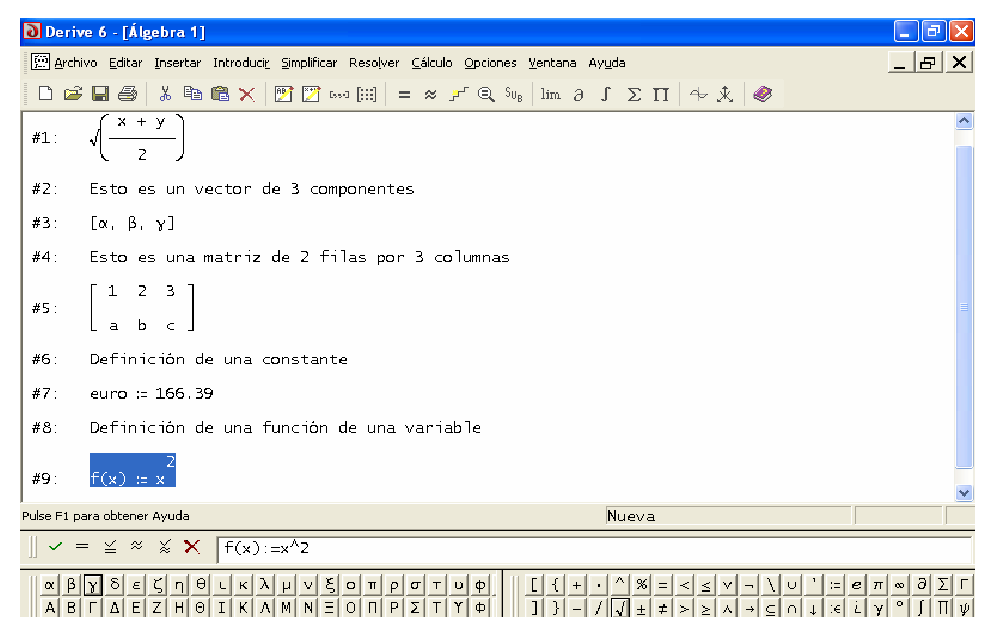
\includegraphics[scale=0.6]{img/introduccion_derive/expresiones}
\caption{Ventana de Algebra con distintos tipos de expresiones.}
\label{g:expresiones}
\end{center}
\end{figure}


\subsection*{Manipulación de archivos}
Las expresiones y los cálculos realizados dentro de la ventana de
Álgebra suelen almacenarse en archivos.

\subsubsection*{Guardar un archivo}
Para crear un archivo donde se guarden las expresiones de la ventana
de Álgebra se utiliza el menú \menu{Archivo>Guardar}, y en el
cuadro de diálogo que aparece se le da nombre al archivo y se
selecciona la carpeta donde queremos guardarlo. Derive le pone
automáticamente la extensión \texttt{*.dfw} a sus archivos. Una vez
creado el archivo, su nombre aparecerá en la barra de título de la
ventana de Derive. Posteriormente, para guardar cambios en una
ventana de Álgebra, bastará con seleccionar de nuevo el menú
\menu{Archivo>Guardar}, de manera que el archivo se actualizará.

\subsubsection*{Recuperar un archivo}
Para recuperar en una ventana de Álgebra el contenido de un archivo
se utiliza el menú \menu{Archivo>Abrir}, y en en cuadro de
diálogo que aparece se selecciona el archivo deseado.
Automáticamente el contenido del archivo aparece en una ventana
nueva de Álgebra.

Otra forma de abrir archivos es mediante el menú
\menu{Archivo>Leer>Math}, que se utiliza para almacenar en
memoria la definición de nuevas funciones, presentes en los archivos
con extensión *.mth, que expanden el potencial de cálculo del núcleo
del programa, el cual queda operativo nada más arrancar Derive. Al
igual que antes aparece un cuadro de diálogo donde debemos
seleccionar el archivo que queremos abrir, sólo que ahora, el
contenido del archivo no aparece en una nueva ventana de Álgebra,
sino que se añade en la ventana de Álgebra activa, a continuación de
las expresiones existentes. Otra forma de proceder con igual
resultado es mediante el menú \menu{Archivo>Leer>Utilidades},
que también permite acceder hasta, y cargar en memoria, los archivos
con extensión *.mth, pero en este caso el conjunto de expresiones
que componen dichos archivos no aparece en la pantalla, aunque sí
que, al estar cargadas en la memoria del ordenador, serán
operativas.

\subsubsection*{Cerrar y abrir nuevas ventanas de Álgebra}
Cuando terminemos una sesión de trabajo, podemos cerrar la ventana
de Álgebra correspondiente mediante el menú
\menu{Archivo>Cerrar}. Por otro lado, en cualquier momento de una
sesión de trabajo podemos abrir, añadidas a la que aparece por
defecto, tantas ventanas de Álgebra como estimemos oportunas
mediante el menú \menu{Archivo>Nuevo}. El programa trabaja con
cada una de las ventanas de Álgebra activas de forma completamente
independiente, lo cual implica, entre otras cosas, que podremos
utilizar los mismos nombres de variables en todas las ventanas
abiertas sin interferencia entre las mismas.

\subsubsection*{Impresión}
Para imprimir el contenido de una ventana de Álgebra, o bien una
gráfica, se utiliza el menú \menu{Archivo>Imprimir}. En el caso
de una ventana de Álgebra aparecerá un cuadro de diálogo donde se
puede seleccionar \texttt{Todo}, para imprimir todo el contenido de
la ventana, \texttt{Páginas} para imprimir un rango de páginas o
\texttt{Selección} para imprimir la zona previamente seleccionada de
la ventana. No obstante, antes de imprimir, conviene utilizar el
menú \menu{Archivo>Vista Previa} para ver por pantalla cómo
quedaría la hoja impresa. Si todo está bien, bastaría con pulsar el
botón \texttt{Imprimir} para que aparezca el cuadro de diálogo de
impresión y desde ahí enviarlo a la impresora. La orientación y los
márgenes pueden cambiarse con el menú \menu{Archivo>Configurar
Página}, mientras que otras opciones como el tipo de letra, o el
encabezado y pie de página se controlan mediante el menú
\menu{Opciones>Impresión>Cabecera y Pie}.

\subsection*{Simplificación de expresiones}
Derive incorpora varios sistemas de simplificación de expresiones.
El más sencillo es la simplificación básica, que puede realizarse
mediante el menú \menu{Simplificar>Normal}. Este menú permite
realizar simplificaciones simples como por ejemplo convertir la
expresión $x+x$ en la expresión $2x$. Sin embargo, no permite pasar
de un binomio como $(x+1)^2$ a su desarrollo $x^2+2x+1$, ya que no
está claro cuál de las dos expresiones es más simple. Para obtener
el desarrollo de este binomio se utiliza el menú
\menu{Simplificar>Expandir} que permite expandir una expresión
con respecto sus variables. Por el contrario, si lo que queremos es
pasar del desarrollo a la forma del binomio, se utiliza el menú
\menu{Simplificar>Factorizar} que permite factorizar una
expresión con respecto a sus variables.

En cualquiera de estas simplificaciones, Derive trabaja por defecto
en modo exacto y por eso devuelve expresiones fraccionarias. Para
obtener el valor de una expresión en modo aproximado, con decimales,
se utiliza el menú \menu{Simplificar>Aproximar}. Con este menú
aparece un cuadro de diálogo donde debemos introducir el número de
decimales que queremos para la aproximación.

Por último, es posible sustituir cualquier variable de una expresión
por un valor u otra expresión mediante el menú
\menu{Simplificar>Sustituir Variable}. En el cuadro de diálogo
que aparece se elige la variable a sustituir y se introduce la
expresión o el valor de sustitución en \texttt{Nuevo Valor}.

\subsection*{Representaciones gráficas}
Derive permite representar gráficamente funciones en 2 y 3
dimensiones.
\subsubsection*{Gráficas en 2 dimensiones}
Para representar una función o expresión de una variable, se
selecciona la expresión y se utiliza el menú \menu{Ventana>Nueva
Ventana 2D}. Automáticamente aparece una ventana de gráficas en 2
dimensiones con unos ejes cartesianos, y para que aparezca la
gráfica de la función, basta con pulsar el menú
\menu{Insertar>Gráfica} de esta ventana, o pulsar en su
correspondiente botón de la barra de botones. En la
figura~\ref{g:2d-plot} se muestra un ejemplo de gráfica en 2
dimensiones.

Si queremos que la gráfica, una vez obtenida, también aparezca en la
ventana de Álgebra como un objeto más de la misma, desde la ventana
2D, utilizamos el menú \menu{Archivo>Incrustar}.

\begin{figure}[h!]
\begin{center}
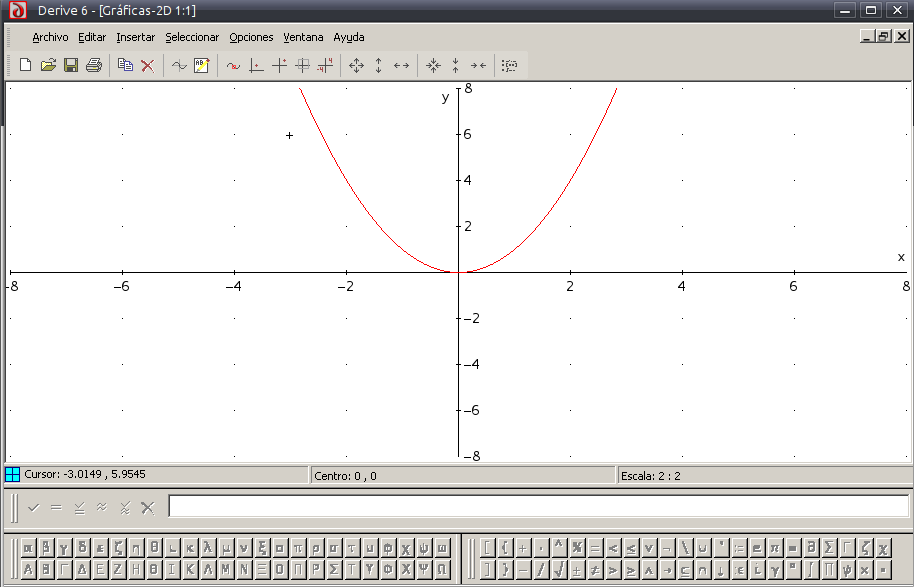
\includegraphics[scale=0.6]{img/introduccion_derive/2d-plot}
\caption{Ventana de gráficas en 2 dimensiones.} \label{g:2d-plot}
\end{center}
\end{figure}

Es posible representar más de una función en una misma gráfica,
seleccionando la nueva expresión en la ventana de Álgebra, y
pulsando de nuevo el menú \menu{Insertar>Gráfica} en la ventana
de gráficos en 2 dimensiones en que queramos que aparezca la
representación gráfica de la expresión seleccionada. Cuando se
quieren representar varias funciones, a veces resulta más cómodo
mostrar al mismo tiempo la ventana de Álgebra y la de gráficas
mediante el menú \menu{Ventana>Mosaico Vertical}, tal y como se
muestra en la figura~\ref{g:expresionesygraficas}.

\begin{figure}[h!]
\begin{center}
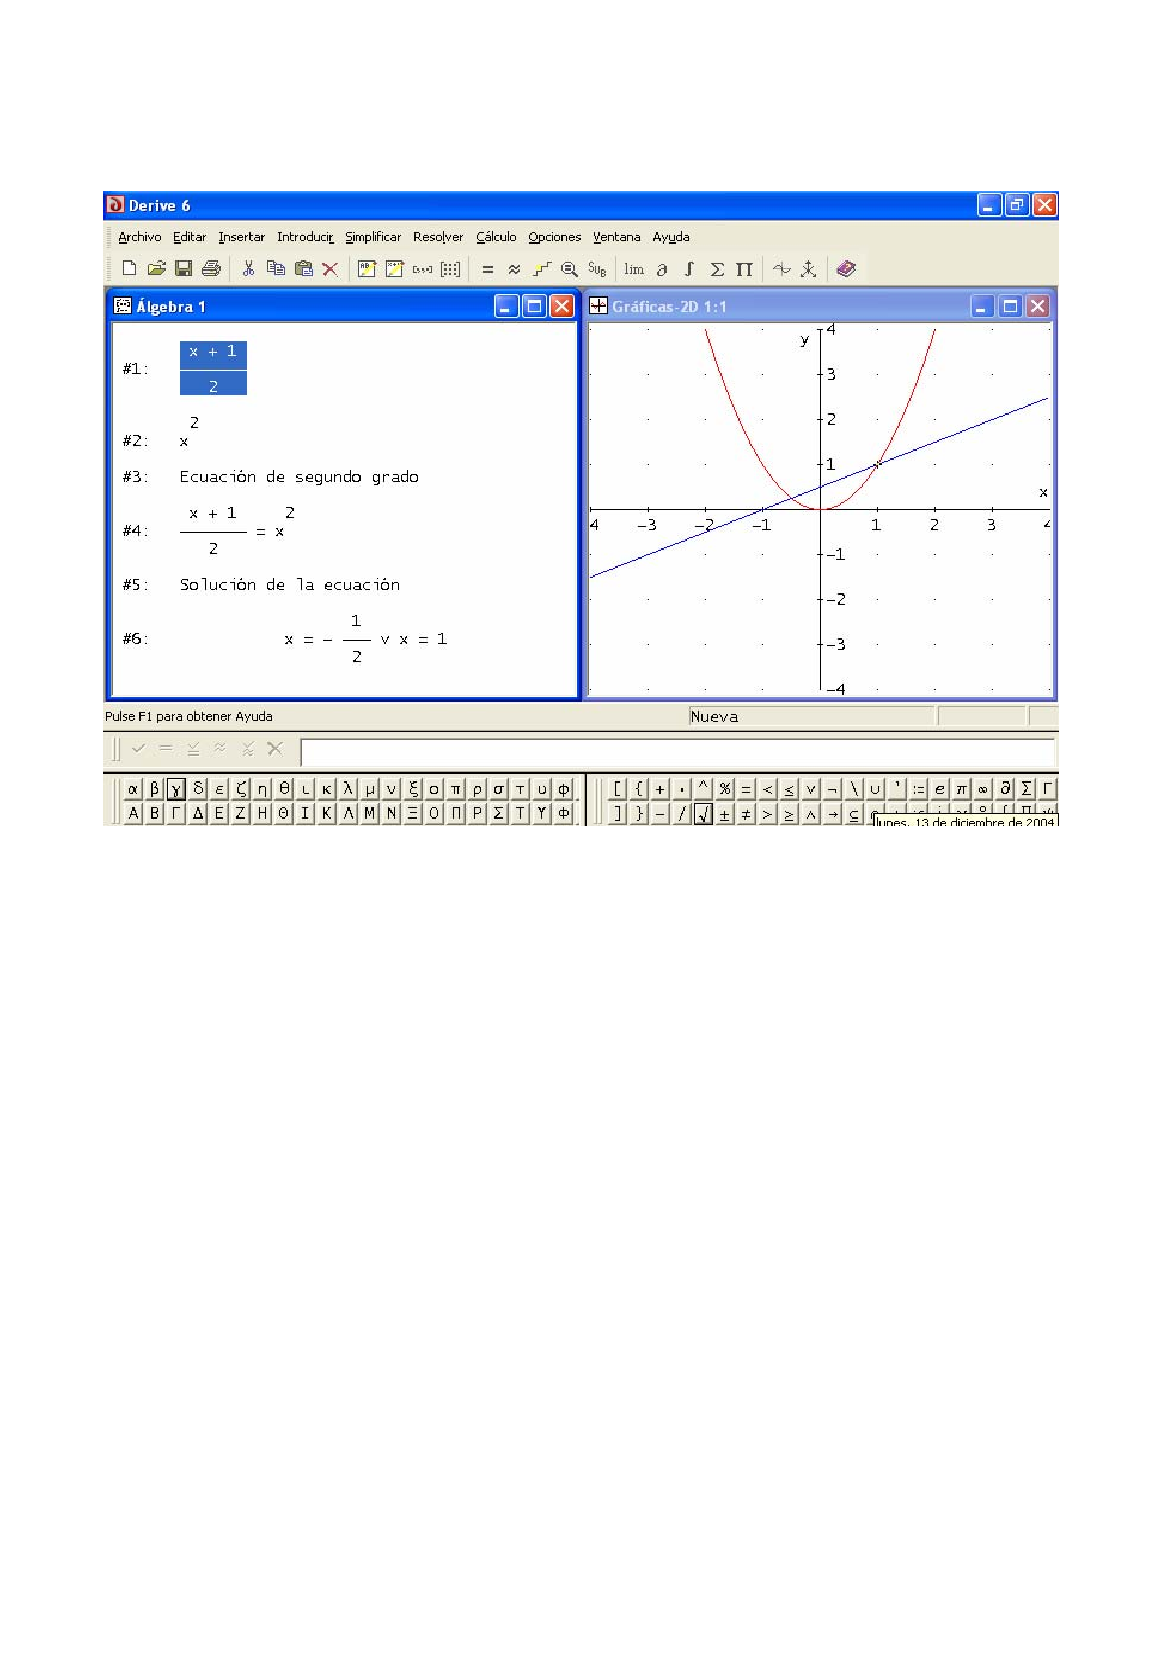
\includegraphics[scale=0.6]{img/introduccion_derive/expresionesygraficas}
\caption{Ventana de Álgebra y de gráficas en 2 dimensiones en una
misma pantalla.} \label{g:expresionesygraficas}
\end{center}
\end{figure}

También es posible borrar gráficas mediante el menú
\menu{Editar>Borrar Gráfica}. Si se elige la opción
\texttt{Primera} se borra la primera gráfica dibujada, si se elige
la opción \texttt{Última} se borra la última, y si se elige la
opción \texttt{Anteriores} borra todas las gráficas excepto la
última.

En la ventana de gráficas en 2 dimensiones existen distintos menús
que permiten cambiar el aspecto de la gráfica representada. Una
posibilidad muy interesante es cambiar la escala de los ejes
mediante el menú \menu{Seleccionar>Relación de Aspecto}.

También es posible ampliar la representación gráfica de una
determinada zona del gráfico mediante el menú
\menu{Seleccionar>Rango de la Gráfica}, introduciendo las
coordenadas de la zona que queremos ampliar, aunque es más práctico
utilizar el botón \texttt{Seleccionar el rango}, y después utilizar
el ratón para delimitar la zona que queremos ampliar.

En la ventana de gráficas en 2 dimensiones aparece una cruz que
representa al cursor. Las coordenadas del cursor siempre aparecen en
la barra de estado. Cuando se pulsa la tecla \texttt{F3}, la cruz se
transforma en un cuadradito y se pasa a \emph{modo de traza}. En
este modo, al mover el cursor con las flechas del teclado, el cursor
sigue la trayectoria de la función representada, con lo que podemos
averiguar los valores que toma la misma en la barra de estado, tal y
como se muestra en la figura~\ref{g:modotraza}.

\begin{figure}[h!]
\begin{center}
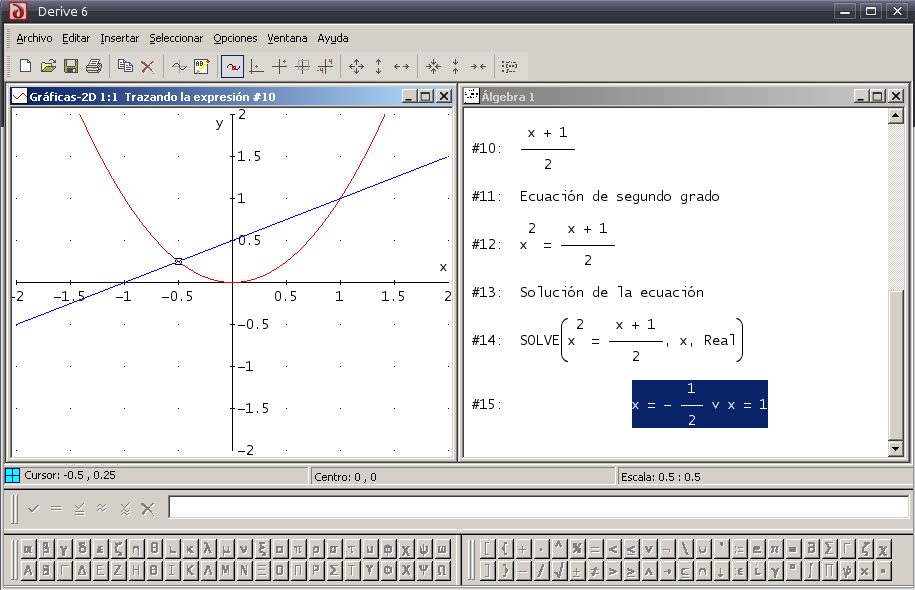
\includegraphics[scale=0.6]{img/introduccion_derive/modotraza}
\caption{Ventana de gráficas en 2 dimensiones en modo de traza con
una gráfica ampliada.} \label{g:modotraza}
\end{center}
\end{figure}

Es posible centrar la gráfica de una función en cualquier punto
mediante el menú \menu{Seleccionar>Rango de la
Gráfica>Longitud/Centro}, aunque, de nuevo, tal vez sea más
operativo hacerlo mediante los botones \texttt{Centrar en el cursor}
y \texttt{Centrar en el origen}.

\subsubsection*{Gráficas en 3 dimensiones}
Para representar una función o expresión de dos variables, se
selecciona la expresión y se utiliza el menú \menu{Ventana>Nueva
Ventana 3D}. Automáticamente aparece una ventana de gráficas en 3
dimensiones con unos ejes cartesianos, y para que aparezca la
gráfica de la función, basta con pulsar el menú
\menu{Insertar>Gráfica} de esta ventana. En la
figura~\ref{g:3d-plot} se muestra un ejemplo de gráfica en 3
dimensiones.

\begin{figure}[h!]
\begin{center}
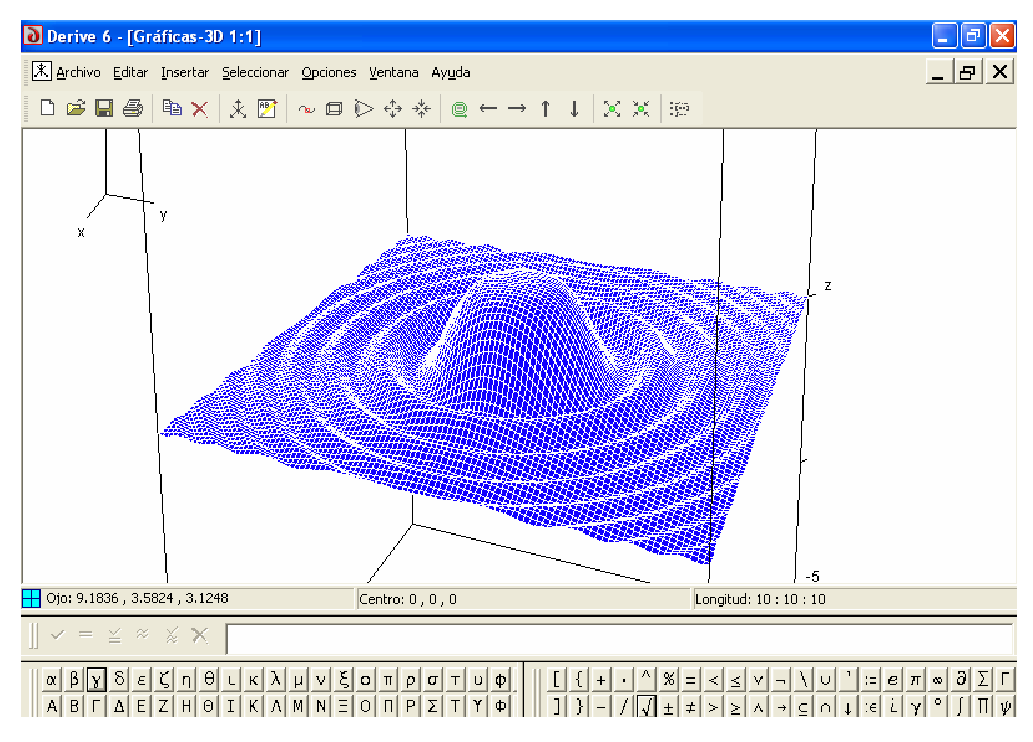
\includegraphics[scale=0.6]{img/introduccion_derive/3d-plot}
\caption{Ventana de gráficas en 3 dimensiones.} \label{g:3d-plot}
\end{center}
\end{figure}

Al igual que en el caso de las gráficas de 2 dimensiones, existen
distintos menús que permiten cambiar el aspecto de la gráfica
representada. De todos ellos, sólo comentaremos el menú
\menu{Editar>Gráfica>Número de Paneles} que permite cambiar la
resolución del gráfico, y el menú \menu{Seleccionar>Posición de
Ojo} que permite cambiar la posición desde donde se mira la gráfica.

